\chapter{Analisis}
\label{chap:analisis}

\section{\textit{Preprocessing} Data Mahasiswa}
\label{sec:preprocessing}
Data mahasiswa yang digunakan adalah data mahasiswa Universitas Katolik Parahyangan dengan jalur penerimaan Penelurusan dan Kemampuan atau PMDK pada tahun 2013-2018. Pada data yang digunakan terdapat beberapa atribut yang tidak dapat digunakan seperti No.PMB,  kota asal sekolah, dan provinsi asal sekolah. Atribut yang tidak dapat digunakan akan dihapus dan data akan dipisahkan menjadi dua \textit{file} mahasiswa dan nilai untuk setiap program studi yang ada. \textit{prepocessing} dilakukkan menggunakan Python. Berikut langkah-langkah dalam \textit{preprocessing} :

\begin{enumerate}
    \item Membaca \textit{file} .csv yang berisikan data mahasiswa pada fakultas tertentu.
    
    \item Membuat tabel untuk data mahasiswa dan nilai. Tabel yang dibuat berupa struktur data dua dimensi yang ukurannya dapat berubah jika ada penambahan data atau pengurangan data. Pembuatan tabel bertujuan untuk menyimpan data mahasiswa dan nilai yang sudah melalui \textit{preprocessing}, yang nantinya data tersebut akan digunakan kedalam basis data.
    
    \item Menginisialisasikan batas \textit{looping}, id\_user, id\_nilai, dan asal jurusan. Pada \textit{file} .csv yang digunakan, setiap mahasiswa memiliki baris sebanyak 4*jumlah mata pelajaran yang digunkan, 4 adalah jumlah semester dari kelas X sampai XII. Data mahasiswa untuk NPM, kode program studi, status, dan IPK terdapat duplikat, batas \textit{looping} digunakan untuk mendapatkan jumlah mahasiswa dengan data yang tidak duplikat, sedangkan id\_user dan id\_nilai digunakan untuk penomoran data yang nantinya akan menjadi \textit{primary key} pada basis data dan asal jurusan digunakan untuk memberikan penenda mahasiswa berasal dari IPA atau IPS. 
    
    \item Menambahkan data mahasiswa berupa NPM, id\_prodi, asal jurusan, dan IPK pada dataframe mahasiswa.
    
    \item Mengubah \textit{range} nilai menjadi GPA (\textit{Grade Point Average}) dan menghitung nilai rata-rata untuk setiap nilai mata pelajaran.
    
    \item Menambahkan data GPA, rata-rata nilai, dan id\_user pada dataframe nilai.
    
    \item Menyimpan tabel mahasiswa dan nilai menjadi .csv.
\end{enumerate}

Hasil \textit{file} .csv nantinya akan di\textit{import} pada basis data yang akan digunakan pada sistem.  

\section{Pemilihan Algoritma Sistem Rekomendasi}
Berdasarkan teori \ref{teknik rekomendasi} yang menjelaskan mengenai teknik-teknik yang dapat digunakan untuk membangun sistem rekomendasi, teknik \textit{collaborative filtering} adalah teknik yang dapat digunakan untuk memberikan rekomendasi berupa program studi kepada calon mahasiswa berdasarkan kesamaan dengan pengguna lain. \textit{Collaborative filtering} menghasilkan rekomendasi item yang spesifik untuk pengguna berdasarkan peringkat tanpa memerlukan informasi tambahan mengenai item ataupun pengguna.

Pada sistem yang dibangun, akan memberikan rekomendasi berdasarkan nilai raport beberapa mata pelajaran siswa pada kelas X dan XI yang digunakan untuk PMDK. Mata pelajaran yang digunakan adalah Matematika, Bahasa Indonesia, Bahasa Inggris, Fisika, Kimia, dan Pendidikan Kewarganegaraan. Rekomendasi program studi berdasarkan asal jurusan saat SMA, misalnya siswa IPA akan diberikan rekomendasi program studi IPA. Setiap jurusan akan menggunakan beberapa mata pelajaran dari mata pelajaran yang disebutkan sebelumnya.

\section{Contoh Pehitungan \textit{Collaborative Filtering}}
\label{subsec:contoh perhitungan}
Pada bagian ini akan diberikan contoh perhitungan dari teknik \textit{collaborative filtering} dengan algoritma \textit{neigihborhood-based} dengan pendekatan \textit{user-based model}. Terdapat dua tahapan dalam penggunaan \textit{user-based model}, yaitu : menghitung kemiripan pengguna dengan pengguna lain dan menghitung prediksi. Perhitungan kemiripan akan menggunakan algoritma \textit{pearson correlation coefficient} dan perhitungan prediksi akan menggunakan algoritma \textit{weighted sum}. Diperlukan data mahasiswa dan data siswa, tabel \ref{tab:data mahasswa} dan tabel \ref{tab:data siswa} merupakan contoh data mahasiswa yang sudah terdapat rata-rata nilai tiap mata pelajaran.

\begin{table}[H]
    \centering
    \renewcommand{\arraystretch}{1.5}
    \begin{tabular}{|l|c|c|c|c|c|}
        \hline
        MP\slash Semester & 101 & 102 & 111 & 112 & AVG \\
        \hline 
        Matematika & 2.6 & 2.9 & 2.95 & 2.75 & 2.8 \\
        \hline 
        Bahasa Indonesia & 0 & 0 & 0 & 0 & 0 \\
        \hline 
        Bahasa Inggris & 2.95 & 3 & 2.85 & 2.95 & 2.9375 \\
        \hline 
        PKN & 0 & 0 & 0 & 0 & 0 \\
        \hline
    \end{tabular}
    \caption{Contoh data mahasiswa dalam bentuk GPA}
	\label{tab:data mahasswa}
\end{table}

\begin{table}[H]
    \centering
    \renewcommand{\arraystretch}{1.5}
    \begin{tabular}{|l|c|c|c|c|c|c|}
        \hline
        MP\slash Semester & 101 & 102 & 111 & 112 & Rumus & AVG \\
        \hline 
        Matematika & 2.9 & 3.4 & 3.4 & 2.9 & $\frac{2.9 + 3.4 +3.4 + 2.9}{4}$ & 3.15 \\
        \hline 
        Bahasa Indonesia & 2.95 & 2.9 & 3.9 & 3.4 & $\frac{2.95 + 2.9 + 3.9 + 3.4}{4}$ & 3.2875 \\
        \hline 
        Bahasa Inggris & 3.3 & 3.35 & 3.25 & 2.9 & $\frac{3.3 + 3.35 + 3.25 + 2.9}{4}$ & 3.2 \\
        \hline 
        PKN & 3.4 & 2.9 & 3.35 & 2.35 & $\frac{3.4 + 2.9 + 3.35 + 2.35}{4}$ & 3 \\
        \hline
    \end{tabular}
    \caption{Contoh data siswa dalam bentuk GPA}
	\label{tab:data siswa}
\end{table}


\subsection{Contoh Perhitungan Kemiripan}
\label{subsec:contoh perhitungan kemiripan}

Terdapat tiga tahapan dalam menghitung kemipiran menggunakan algoritma \textit{pearson correlation coeficient}, yaitu :

\begin{enumerate}
    \item Menhitung Kovariasi Mahasiswa dan Siswa\\
        \begin{table}[H]
            \centering
            \renewcommand{\arraystretch}{1.5}
            \begin{tabular}{|c|c|c|c|c|}
                \hline
                No & Rumus & Matematika & Rumus & Bahasa Inggris \\
                \hline
                \multirow{2}{*}{1} & $(2.9-3.15)*$ & 0.5    & $(3.3-3.2)*$ & 0.00125\\
                & $(2.6-2.8)$ & & $(2.95-2.9375)$ &  \\
                \hline
                \multirow{2}{*}{2} & $(3.4-3.15)*$ & 0.025  & $(3.35-3.2)*$ & 0.009375 \\
                & $(2.9-2.8)$ & & $(3-2.9375)$ &  \\
                \hline
                \multirow{2}{*}{3} & $(3.4-3.15)*$ & 0.0375 & $(3.25-3.2)*$ & -0.004375 \\
                & $(2.95-2.8)$ &  & $(2.85-2.9375)$ &  \\
                \hline
                \multirow{2}{*}{4} & $(2.9-3.15)*$ & 0.0125 & $(2.9-3.2)*$ & -0.00375 \\
                & $(2.75-2.8)$ &  & $(2.95-2.9375)$ &  \\
                \hline
                \multirow{2}{*}{Sigma} & $0.5 + 0.025 +$ & 0.125 & $0.00125 + 0.009375 +$ & 0.0025 \\
                & $0.0375 + 0.0125$ & & $-0.004375 + -0.00375$ &  \\
                \hline
                \multicolumn{3}{|c|}{Hasil} & $0.125+0.0025$ & 0.1274 \\
                \hline
            \end{tabular}
            \caption{Nilai kovariasi mahasiswa dan siswa}
            \label{tab:kovariasi}
        \end{table}
        
        \item Menghitung Standar Deviasi Mahasiswa dan Siswa \\
            \begin{table}[H]
                \centering
                \renewcommand{\arraystretch}{1.5}
                \begin{tabular}{|c|c|c|c|c|}
            		\hline
            		No & Rumus & Matematika & Rumus & Bahasa Inggris\\
            		\hline
            		1 & $(2.6-2.8)^2$ & 0.04 & $(2.95-2.9375)^2$ & 0.00015625 \\
            		\hline
            		2 & $(2.9-2.8)^2$ & 0.01 & $(3-2.9375)^2$ & 0.00390625 \\
            		\hline
            		3 & $(2.95-2.8)^2$ & 0.0225 & $(2.85-2.9375)^2$ & 0.00765625 \\
            		\hline
            		4 & $(2.75-2.8)^2$ & 0.0225 & $(2.95-2.9375)^2$ & 0.00015625
             \\
            		\hline
            		\multirow{2}{*}{Sigma} & 0.04+0.01+ & 0.075 & 0.0.000156250.00390625+ & 0.011875\\
            		& 0.0225+0.0225 & & 0.00765625+0.00015625 & \\
            		\hline
            		\multicolumn{3}{|c|}{Hasil} & $\sqrt{0.075+0.011875}$ & 0.294745653	 \\
            		\hline
                \end{tabular}
                \caption{Standar Deviasi Mahasiswa}
            	\label{tab:sd_mahasiswa}
            \end{table}
            
            \begin{table}[H]
                \centering
                \renewcommand{\arraystretch}{1.5}
                \begin{tabular}{|c|c|c|c|c|}
            		\hline
            		No & Rumus & Matematika & Rumus & Bahasa Inggris\\
            		\hline
            		1 & $(2.9-3.15)^2$ & 0.0625 & $(3.3-3.2)^2$ & 0.01 \\
            		\hline
            		2 & $(3.4-3.15)^2$ & 0.0625 & $(3.35-3.2)^2$ & 0.0225 \\
            		\hline
            		3 & $(3.4-3.15)^2$ & 0.0625 & $(3.25-3.2)^2$ & 0.0025 \\
            		\hline
            		4 & $(2.9-3.15)^2$ & 0.0625 & $(2.9-3.2)^2$ & 0.09 \\
            		\hline
            		\multirow{2}{*}{Sigma} & 0.0625+0.0625+ & 0.25 & 0.01+0.0225+ & 0.125\\
            		& 0.0625+0.0625 & & 0.0025+0.09 & \\
            		\hline
            		\multicolumn{3}{|c|}{Hasil} & $\sqrt{0.25+0.125}$ & 0.612372436 \\
            		\hline
                \end{tabular}
                \caption{Standar Deviasi Siswa}
            	\label{tab:sd_siswa}
            \end{table}
            
        \item Menghitung kemiripan \\
            \begin{table}[H]
                \centering
                \renewcommand{\arraystretch}{1.5}
                \begin{tabular}{|c|c|c|c|}
                    \hline
                    No & Rumus & Kemiripan & IPK \\ 
                    \hline
                    1 & $\frac{0.1275}{0.612372436*0.294745653}$ & 0.706394228 & 3.11\\
                    \hline
                    2 & $\frac{0.0125}{0.612372436*0.2343242}$ & 0.08711185 & 2.9 \\
                    \hline
                    3 & $\frac{0.2}{0.612372436*0.543242}$ & 0.601202838 & 3 \\
                    \hline
                    4 & $\frac{0.125}{0.612372436*0.432343}$ & 0.472134729 & 3.2\\
                    \hline
                    5 & $\frac{0.05}{0.612372436*0.242345}$ & 0.336914969 & 3.4\\
                    \hline
                \end{tabular}
                \caption{Contoh Perhitungan Kemiripan}
                \label{tab:kemiripan}
            \end{table}
\end{enumerate}

Setelah melakukan ketiga tahapan tersebut, nilai kemiripan pada tabel \ref{tab:kemiripan} akan dipilih nilai kemiripan yang bernilai lebih besar dari 0, karena jika nilai kemiripan mendekat -1, mahasiswa tersebut dapat dikatakan tidak memiliki kemiripan denga pengguna,  maka nilai kesamaan pada tabel \ref{tab:kemiripan} semuanya dapat digunakan untuk prediksi.


\subsection{Contoh Perhitungan Prediksi}
\label{subsec:contoh perhitungan prediksi}

Setelah melakukan perhitungan kemiripan antara mahasiswa dan siswa, tahapan selanjutnya adalah menghitung prediksi IPK. Berikut merupakan contoh dari perhitungan prediksi :

\begin{table}[H]
    \centering
    \renewcommand{\arraystretch}{1.5}
    \begin{tabular}{|c|c|c|c|}
        \hline
        No & Kesamaan & Rumus & Kesamaan*IPK \\
        \hline
        1 & 0.706394228 & 0.706394228*3.11 & 2.196886049 \\
        \hline
        2 & 0.08711185 & 0.08711185*2.9 &  0.252624364 \\
        \hline
        3 & 0.601202838 & 0.601202838*3 & 1.803608514 \\
        \hline
        4 & 0.472134729 & 0.472134729*3.2 & 1.510831133 \\
        \hline
        5 & 0.336914969 & 0.336914969*3.4 & 1.145510893 \\
        \hline
        Sigma & 2.203758614 & - & 6.909460954 \\
        \hline
        \multicolumn{2}{|c|}{Hasil} & $\frac{6.909460954}{2.203758614}$ & 3.13530752\\
        \hline
    \end{tabular}
    \caption{Contoh hasil Prediksi}
    \label{tab:prediksi}
\end{table}

\section{Contoh Perhitungan Metode Evaluasi Sistem Rekomendasi}
\label{sec:contoh perhitungan evaluasi}

Berdasarkan penjelasan mengenai sistem rekomendasi yang dibahas pada bab \ref{chap:landasan teori} bagian \ref{sec:aplikasi dan evaluasi}. Salah satu bagian terpenting adalah evaluasi. Evalusi pada sistem rekomendasi dilakukkan untuk mendapatkan akurasi dari hasil prediksi yang diberikan. Akurasi merupakan salah satu aspek yang sering dijadikan acuan untuk rekomendasi yang digunakan. Dalam melakukan pengujian akurasi bisa menggunkan metode \textit{Mean Absolute Error} (MAE) dan \textit{Root Mean Square Error} (RMSE). Berikut merupakan contoh penerapan kedua metode yang akan disajikan dalam tabel \ref{tab:tabel data mae dan rmse} :

\begin{longtable}[H]{|c|c|c|c|c|c|c|c|}
    %\centering
    %\begin{tabular}{|c|c|c|c|c|c|c|c|}
        \hline
        \multirow{2}{2em}{No} & Item & Pengguna & Penilaian Asli & Prediksi Sistem  & $r_{u,i}-\hat{r}_{u,i}$ & $\mid r_{u,i}-\hat{r}_{u,i} \mid$ & $(r_{u,i}-\hat{r}_{u,i})^2$ \\ 
        & & & $r_{u,i}$ & $\hat{r}_{u,i}$ & & &\\
        \hline
        1 & 110 & 1 & 3.4 & 3.5 & -0.1 & 0.1 & 0.01\\
        \hline
        2 & 120 & 30 & 3.3 & 3.1 & 0.2 & 0.2 & 0.04\\
        \hline
        3 & 130 & 56 & 3 & 2.8 & 0.2 & 0.2 & 0.04\\
        \hline
        4 & 200 & 65 & 2.9 & 3.1 & -0.2 & 0.2 & 0.04\\
        \hline
        5 & 310 & 76 & 3.1 & 2.8 & 0.3 & 0.3 & 0.09\\
        \hline
        6 & 320 & 87 & 3.2 & 3 & 0.2 & 0.2 & 0.04\\
        \hline
        7 & 330 & 99 & 2.8 & 3 & -0.2 & 0.2 & 0.04\\
        \hline
        8 & 410 & 102 & 3.4 & 3.5 & -0.1 & 0.1 & 0.01\\
        \hline
        9 & 420 & 167 & 3.1 & 3.5 & -0.4 & 0.4 & 0.16\\
        \hline
        10 & 510 & 189 & 2.8 & 3.1 & -0.3 & 0.3 & 0.09\\
        \hline
        11 & 610 & 298 & 3.1 & 2.9 & 0.2 & 0.2 & 0.04\\
        \hline
        12 & 620 & 344 & 3.4 & 2.9 & 0.5 & 0.5 & 0.25\\
        \hline
        13 & 630 & 365 & 3.1 & 3 & 0.1 & 0.1 & 0.01\\
        \hline
        14 & 710 & 465 & 2.9 & 3 & -0.1 & 0.1 & 0.01\\
        \hline
        15 & 720 & 477 & 3.4 & 3.5 & -0.1 & 0.1 & 0.01\\
        \hline
        16 & 730 & 480 & 3.4 & 3.6 & -0.2 & 0.2 & 0.04\\
        \hline
        \multicolumn{6}{|c|}{Jumlah} & 3.4 & 0.92 \\
        \hline
    %\end{tabular}
    \caption{Tabel Data MAE dan RMSE}
    \label{tab:tabel data mae dan rmse}
\end{longtable}

Berdasarkan data pada tabel \ref{tab:tabel data mae dan rmse} jika dihitung dengan persamaan MAE seperti yang dijelaskan pada \ref{sec:aplikasi dan evaluasi} dengan rumus \ref{rumus mae} maka akan didapatkan hasil pengimplementasian dari rumus MAE sebagai berikut :

\begin{equation}
    MAE = \frac{1}{16} * 3.4 = 0.2125 
\end{equation}

Berdasarkan data pada tabel \ref{tab:tabel data mae dan rmse} jika dihitung dengan persamaan RMSE seperti yang dijelaskan pada \ref{sec:aplikasi dan evaluasi} dengan rumus \ref{rumus rmse} maka akan didapatkan hasil pengimplementasian dari rumus RMSE sebagai berikut :

\begin{equation}
    RMSE = \sqrt{\frac{1}{16} * 0.91} = 0.0575
\end{equation}

\section{Analisis Perangkat Lunak Sejenis}
\label{sec:analisis pl}

Salah satu \textit{website} yang dapat memberikan rekomendasi program studi adalah \url{https://rencanamu.id}. Sistem tersebut dikembangkan menggunakan riset ilmiah, Rencanamu mengukur 7 dimensi profil siswa sebagai landasan dalam rekomendasi, perencanaan kuliah dan karier yang terintegrasi, berkesinambungan dan menyeluruh. Gambar \ref{fig:7 dimensi siswa} menunjukkan 7 dimensi profil siswa. % https://rencanamu.id/about-us

\begin{figure}[H]
    \centering
    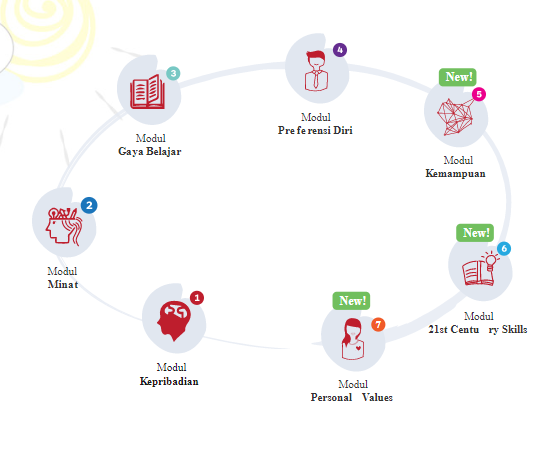
\includegraphics[width = 12cm, height = 12cm]{Gambar/gambar31.PNG}
    \caption{7 Dimensi Profil Siswa}
    \label{fig:7 dimensi siswa}
\end{figure}

Pada sistem ini, telah dilakukan beberapa analisis dan hasilnya sebagai berikut :

\begin{enumerate}
    \item \textit{Website} \url{https://rencanamu.id} adalah sebuah \textit{platform} persiapan kuliah dan karier \textit{online} berbasis data didukung oleh teknologi \textit{People Science} untuk membantu siswa dalam merancang dan mempersiapkan masa depan mereka. 
    
    \item Perlu melakukan registrasi atau \textit{login} kedalam sistem. Terdapat lima \textit{role} pengguna saat melakukan registrasi, yaitu : Siswa SMP, Siswa SMA, Siswa SMK, Mahasiswa, dan Alumni. Setelah memilih role, pengguna diminta untuk mengisi rencana yang akan di buat, terdapat dua pilihan yaitu : Rencana Siap Kuliah dan Rencana Siap Kerja.
    
    \item Gambar \ref{fig: tampilan setelah regis atau login} merupakan tampilan awal setelah registrasi atau \textit{login}. Tampilan ini merupaka tampilan pengguna yang melakukan registrasi sebagai siswa SMA. Tampilan tersebut sama seperti pengguna yang melakukan registrasi sebagai Siswa SMP atau SMK, sedangkan jika pengguna registrasi sebagai mahasiswa atau alumni akan berbeda.
    
    \begin{figure}[H]
        \centering
        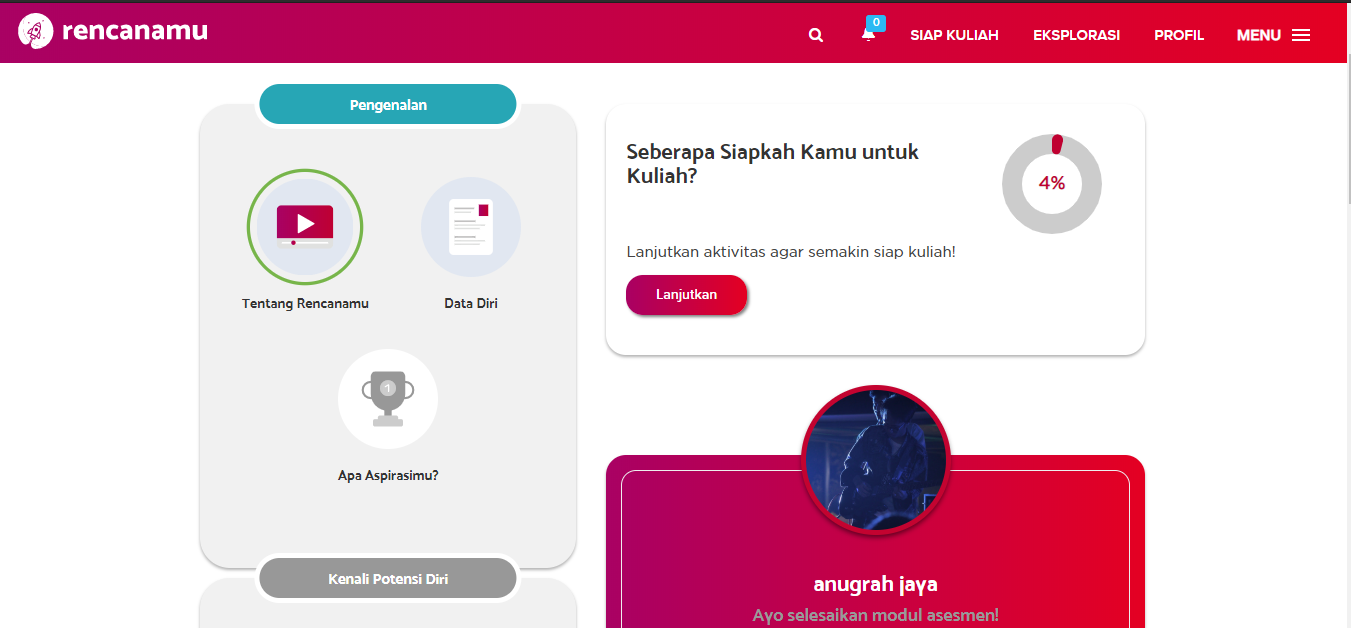
\includegraphics[width = 10cm, height = 6 cm]{Gambar/gambar32.PNG}
        \caption{Tampilan setelah registrasi atau \textit{login}}
        \label{fig: tampilan setelah regis atau login}
    \end{figure}
    
    \item Terdapat tiga modul yang harus dikerjakan oleh penggunan, yaitu modul pengenalan seperti pada gambar \ref{fig:modul pengenalan}, modul kenali potensi diri seperti pada gambar \ref{fig:modul potensi diri}, dan modul ukur kemampuan diri seperti pada gambar \ref{fig:modul ukuran kemampuan diri}. Pada setiap modul terdapat beberapa sub-modul yang harus diselesaikan, jika sub-modul sudah dikerjakan akan muncul lingkaran hijau pada sub-modul. Pengerjaan modul harus dilakukan satu persatu, karena modul kenali potensi diri tidak dapat dikerjakan jika modul pengenalan belum diselesaikan, begitu juga dengan modul ukur kemampuan diri tidak dapat dikerjakan jika modul kenali potensi diri belum diselesaikan.
    
    \item Gambar \ref{fig:modul pengenalan} merupakan modul pertama yang harus dikerjakan, yaitu modul pengenalan. Terdapat 3 sub-modul, yaitu : 
    \begin{enumerate}
        \item Tentang Rencanamu \\
            Sub-modul ini merupakan sebuah video yang menjelaskan mengenai \textit{website} \url{rencanamu.id} dengan durasi 35 detik.
            
        \item Data Diri \\
            Pada sub-modul ini, pengguna diminta untuk mengisi data diri, seperti :
            \begin{enumerate}
                \item Jenis Kelamin \\
                    Pada bagian ini diberikan dua pilihan jenis kelamin, yaitu : laki-laki dan perempuan.
                    
                \item Tanggal Lahir\\
                    Pada bagian ini berikan \textit{text field} untuk mengisi tanggal lahir, dengan format DD-MM-YYYY.
                    
                \item Asal Sekolah \\
                    Pada bagian ini terdapat \textit{dropdown} untuk memilih sekolah yang sudah terdaftar didalam sistem dan terdapat \textit{search bar} untuk membantu memudahkan pencarian. Jika asal sekolah belum terdaftar pengguna dapat menambahkan sekolah tersebut kedalam sistem.
                    
                \item Kelas dan Jurusan \\
                    Pada bagian ini terdapat \textit{dropdown} untuk memilih kelas, terdapat tiga pilihan, yaitu : X, XI, dan XII. Sedangkan untuk jurusan terdapat 4 pilihan, yaitu : IPA, IPS, Bahasa dan Kejurusan, untuk kejurusan terdapat \textit{dropdown} untuk memilih kejurusan yang sudah terdaftar didalam sistem dan terdapat \textit{search bar} untuk membantu memudahkan pencarian. Jika kejurusan belum terdaftar pengguna dapat menambahkan sekolah tersebut kedalam sistem.
                    
                \item Ekstrakurikuler di Sekolah \\
                    Pada bagian ini terdapat \textit{text field} yang diberikan \textit{suggestion} untuk ekstrakurikuler yang terdaftar pada sistem, ekstrakurikuler yang diisi bisa lebih dari satu dan jika ekstrakurikuler belum terdaftar pengguna dapat menambahkan sekolah tersebut kedalam sistem. Terdapat pilihan jika tidak mengikuti ekstrakurikuler.
                    
                \item Alamat dan Nomor Telepon \\
                    Pada bagian ini terdapat \textit{dowpdown} untuk memilih kota atau kabupaten yang terdaftar  pada sistem, terdapat \textit{search bar} untuk membantu memudahkan pencarian dan \textit{text field} untuk mengisi nomor telepon.
            \end{enumerate}
        
        \item Apa Aspirasimu ? \\
            Menurut KBBI, aspirasi adalah harapan dan tujuan untuk keberhasilan pada masa yang akan datang. Pada sub-modul ini pengguna diminta untuk mengisi beberapa hal yang sesuai dengan keinginan pengguna, seperti :
            \begin{enumerate}
                \item Bidang yang diinginkan \\
                    Pada bagian ini pengguna diminta untuk memilih bidang apa yang pengguna inginkan. Terdapat beberapa pilihan bidang yang sudah disediakan oleh sistem, pengguna dapat memilih lebih dari satu bidang, jika pengguna belum mengetahui bidang apa yang diinginkan, terdapat pilihan "Belum Tahu".
                    
                \item Profesi yang diinginkan \\
                    Pada bagian ini pengguna diminta untuk memilih profesi apa yang pengguna inginkan. Terdapat \textit{text field} untuk mengisi profesi yang diinginkan, \textit{text field} diberikan \textit{suggestion}. Terdapat pilihan profesi popurel yang sudah disediakan oleh sistem, pengguna dapat memilih lebih dari satu profesi jika pengguna belum mengetahui profesi apa yang diinginkan, terdapat pilihan "Belum Tahu".
                    
                \item Jurusan yang diinginkan \\
                    Pada bagian ini pengguna diminta untuk memilih jursan apa yang pengguna inginkan saat melanjutkan diperguruan tinggi. Terdapat \textit{text field} untuk mengisi jurusan yang diinginkan, \textit{text field} diberikan \textit{suggestion}. Terdapat pilihan jurusan yang sudah disediakan oleh sistem, pengguna dapat memilih lebih dari satu jurusan jika pengguna belum mengetahui jurusan apa yang diinginkan, terdapat pilihan "Belum Tahu".
                 
                \item Pelajaran yang disukai\\
                    Pada bagian ini pengguna diminta untuk memilih mata pelajaran apa yang disukai pengguna.  Terdapat \textit{text field} untuk mengisi pelajaran yang disukai, \textit{text field} diberikan \textit{suggestion}. Terdapat pilihan pelajaran yang sudah disediakan oleh sistem, pengguna dapat memilih lebih dari satu pelajaran yang disukai.
                    
                \item Jenis perguruan tinggi yang diinginkan\\
                    Pada bagian ini pengguna diminta untuk memilih jenis perguruan tinggi yang diinginkan, terdapat empat pilihan, yaitu : perguruan tinggi negeri, perguruan tinggi swasta, perguruan tinggi kedinasan, dan perguruan tinggi keagamaan islam negeri. Pengguna dapat memilih lebih dari jenis perguruan tinggi.
                    
                \item Kampus yang diinginkan \\
                    Pada bagian ini pengguna diminta untuk memilih perguruan tinggi yang pengguna inginkan. Terdapat \textit{text field} untuk mengisi perguruan tinggi yang diinginkan, \textit{text field} diberikan \textit{suggestion}. Terdapat pilihan perguruan tinggi yang sudah disediakan oleh sistem, pengguna dapat memilih lebih dari satu perguruan tinggi jika pengguna belum mengetahui perguruan tinggi apa yang diinginkan, terdapat pilihan "Belum Tahu".
                    
                \item Kesediaan kuliah di luar kota \\
                    Pada bagian ini pengguna diminta untuk menjawab pertanyaan "Apakah kamu bersedia kuliah diluar kota?", terdapat tiga jawaban untuk dipilih, yaitu : bersedia, tidak bersedia, belum tahu.
                    
                \item Peryataan mengikuti bimbel \\
                    Pada bagian ini pengguna diminya untuk menjawab pertayaan "Apakah kamu megikuti bimbel?", terdapat empat jawaban untuk dipilih, yaitu : pernah dan sudah berbenti, tidak pernah, sedang mengikuti, berencana mengikuti. Jika memilih jawaban pernah dan sudah berhenti, akan diminta untuk mengisi bimbel apa yang pernah diikuti.
                    
                \item Informasi mengenai beasiswa\\
                    Pada bagian ini pengguna diminta untuk menjawab pertanyaan "Apakah kamu tertarik mendapatkan informasi beasiswa?", terdapat empat jawaban yang dapat dipilih, yaitu : iya beasiswa dalam negeri, iya beasiswa luar negeri, iya keduanya, dan tidak.
                    
                \item Uang saku perhari\\
                    Pada bagian ini pengguna diminta untuk mengisi berapa uang saku yang diterima perhari, terdapat empat pilihan untuk dipilih, yaitu : dibawah 10 ribu, 11 - 25 ribu, 26 - 50 ribu, dan diatas 50 ribu.
                    
                \item Pekerjaan orang tua\\
                    Pada bagian ini pengguna diminta untuk mengisi pekerjaan orang tua dengan pilihan yang sudah disediakan oleh sistem.
                    
                \item Penghasilan orang tua\\
                    Pada bagian ini pengguna diminta untuk mengisi penghasilan orang tua dengan pilihan yang sudah disediakan oleh sistem dalam bentuk \textit{range}.
                    
                \item Jumalah saudara \\
                    Pada bagain ini pengguna diminta untuk mengisi berapa jumlah saudara yang dimiliki beserta dengan dirinya.
                
            \end{enumerate}
    \end{enumerate}
    
    \begin{figure}[H]
        \centering
        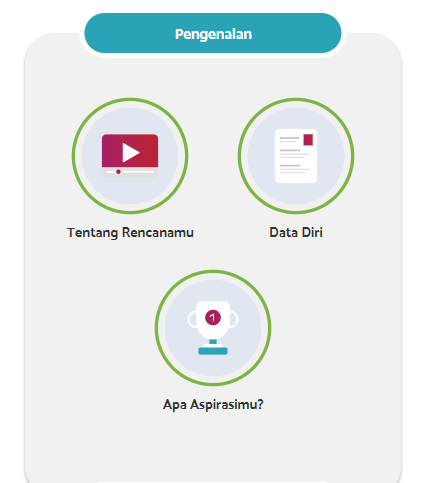
\includegraphics[width = 7cm, height = 10cm ]{Gambar/gambar33.PNG}
        \caption{Modul Pengenalan}
        \label{fig:modul pengenalan}
    \end{figure}
    
    \item Gambar \ref{fig:modul potensi diri} merupakan modul kedua setelah model pengenalan, yaitu modul kenali potensi diri. Terdapat 8 sub-modul, yaitu :
    \begin{enumerate}
        \item Kepribadian \\
            Sub-modul ini merupakan video dengan materi mengenali kepribadian dengan durasi 1 menit. 
            
        \item Tes Kepribadian \\
            Sub-modul ini merupakan tes untuk mengetahui kepribadian pengguna, terdapat beberapa peryantaan yang terdiri dari dua pilihan. Pengguna diminta untuk memilih jawaban yang mendekati atau paling menggambarkan diri pengguna. Terdapat 40 pernyataan yang harus dipilih. Hasil tes akan ditampilkan setelah tes selesai dikerjakan. Pada gambar \ref{fig:hasil tes kepribadian} merupakan contoh dari hasil tes keperibadian.
            
            \begin{figure}[H]
                \centering
                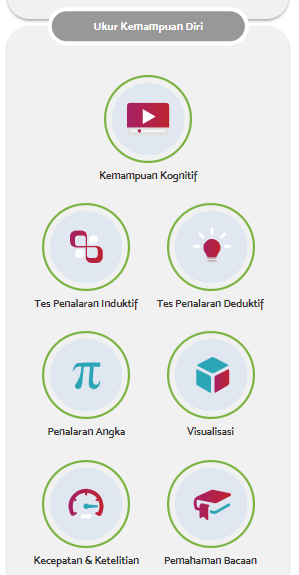
\includegraphics[width = 10cm, height = 12cm]{doc/DokumenSkripsi/Gambar/gambar35.PNG}
                \caption{Hasil Tes Kepribadian}
                \label{fig:hasil tes kepribadian}
            \end{figure}
            
        \item Minat \\
             Sub-modul ini merupakan video dengan materi mengenali minat dengan durasi 54 detik. 
            
        \item Tes Minat \\
            Sub-modul ini merupakan test untuk mengetahui minat pengguna, terdapat beberapa pertanyaan dengan dua pilihan jawaban, yaitu suka dan tidak suka. Pengguna diminta untuk menjawab dengan memilih jawaban yang sesuai dengan minat pengguna. Terddapat beberapa teme, yaitu : kegiatan yang disukai dengan jumlah pertanyaan sebanyak 60, kegiatan yang dapat dilakukan dengan baik dengan jumlah pertanyaan sebanyak 60, topik yang diminati dengan jumlah pertanyaan sebanyak 60, dan profesi yang diminati dengan jumlah pertanyaan sebanyak 60. Hasil tes akan ditampilkan setelah tes selesai dikerjakan. Pada gambar \ref{fig:hasil tes minat} merupakan contoh dari hasil tes minat.
            
            \begin{figure}[H]
                \centering
                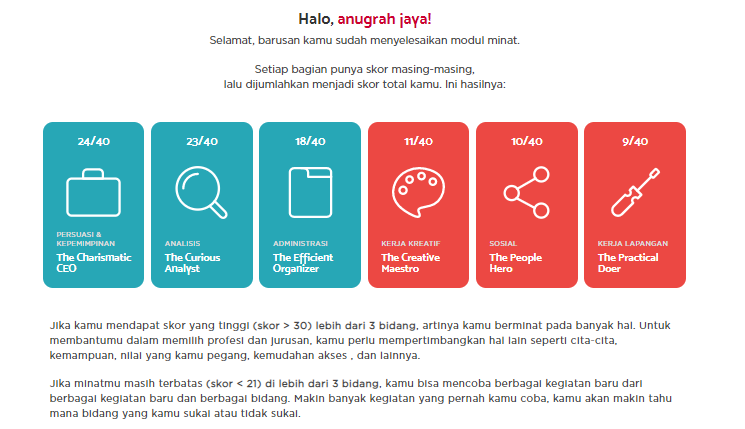
\includegraphics[width = 12cm, height = 10cm]{doc/DokumenSkripsi/Gambar/gambar36.PNG}
                \caption{Hasil Tes Minat}
                \label{fig:hasil tes minat}
            \end{figure}
        
        \item Gaya Belajaran \\
            Sub-modul ini merupakan video dengan materi menganali gaya pelajar dengan durasi 49 detik.
            
        \item Tes Gaya Belajaran \\
            Sub-modul ini merupakan test untuk mengetahui gaya belajar pengguna, terdapat beberapa pernyataan dengan pilihan jawaban suka sekali, suka, dan biasa saja untuk modul 3-1 dan 3-2, sedangkan untuk modul 3-3 terdapat 5 pilihan sesuai dengan kontek yang ditanyakan.. Pengguna diminta untuk memilih jawaban yang sesuai dengan pengguna. Terdapat beberapa tema, yaitu : 3-1 modul gaya belajar dengan jumlah pernyataan 18, 3-2 modul gaya belajar dengan jumlah pernyataan 18, 3-3 Modul gaya belajar dengan jumlah pernyataan 14. Hasil tes akan ditampilkan setelah tes selesai dikerjakan. Pada gambar \ref{fig:hasil tes gaya belajar} merupakan contoh dari hasil tes gaya belajar.
            
            \begin{figure}[H]
                \centering
                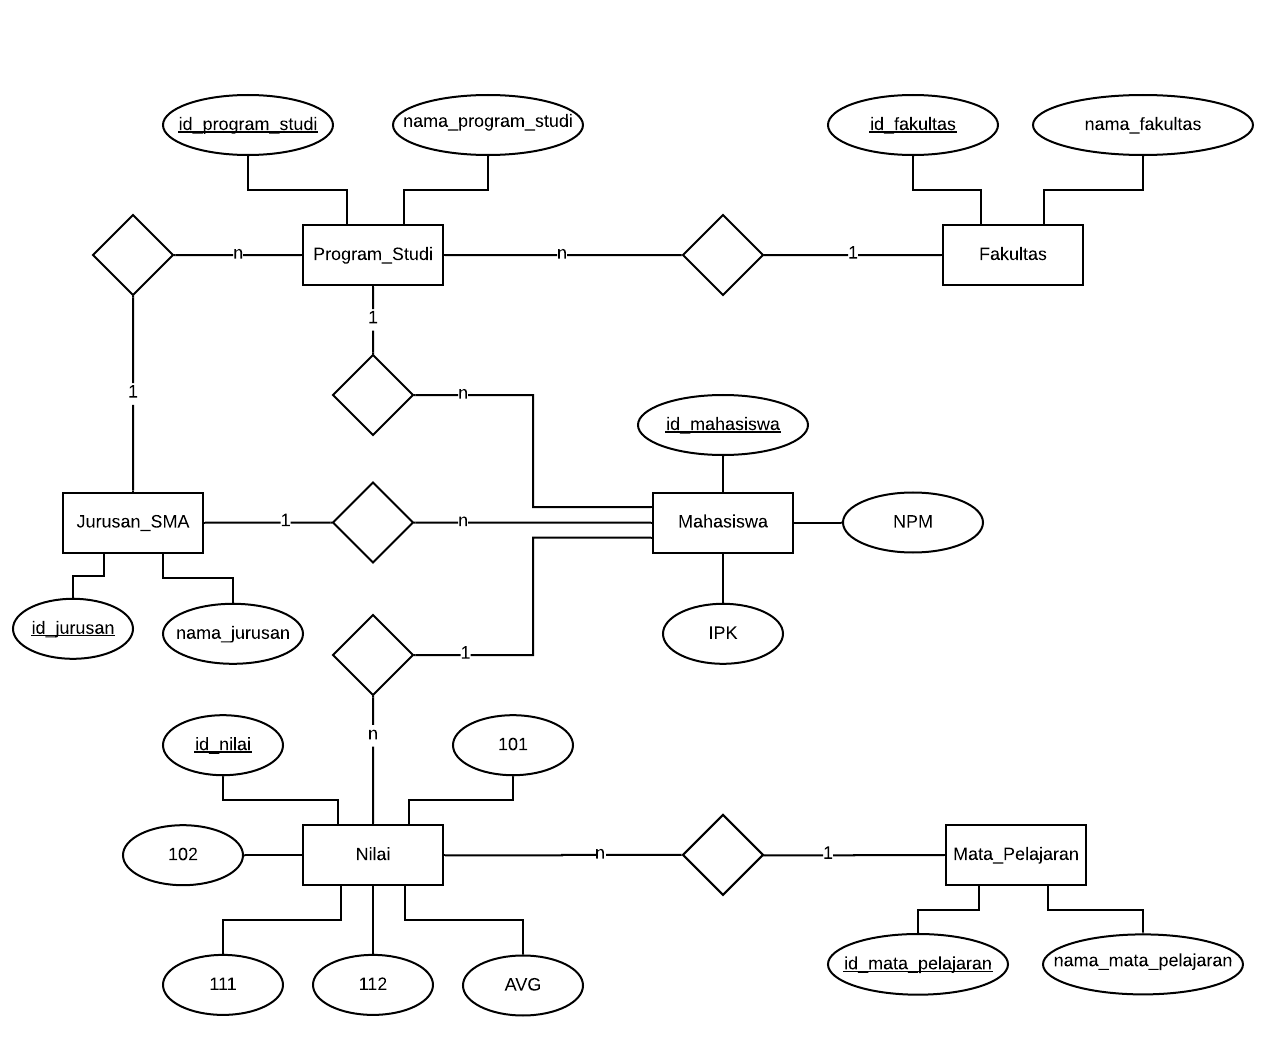
\includegraphics[width = 8cm, height = 10cm]{doc/DokumenSkripsi/Gambar/gambar37.PNG}
                \caption{Hasil Tes Gaya Belajar}
                \label{fig:hasil tes gaya belajar}
            \end{figure}
            
        \item \textit{Personal Values} \\
            Sub-modul ini merupakan video dengan materi mengenali \textit{personal values} dengan durasi 1 menit 1 detik. Hasil tes akan ditampilkan setelah tes selesai dikerjakan.
            
        \item Tes \textit{Personal Values} \\
            Sub-modul ini merupakan test untuk mengetahui \textit{personal values} pengguna, terdapat 45 pasang pernyataan. Pengguna diminta untuk memilih salah satu dari dua peryantaan yang diberikan. Hasil tes akan ditampilkan setelah tes selesai dikerjakan. Hasil tes akan ditampilkan setelah tes selesai dikerjakan. Pada gambar \ref{fig:hasil tes personal values} merupakan contoh dari hasil tes \textit{personal values}. 
            
            \begin{figure}[H]
                \centering
                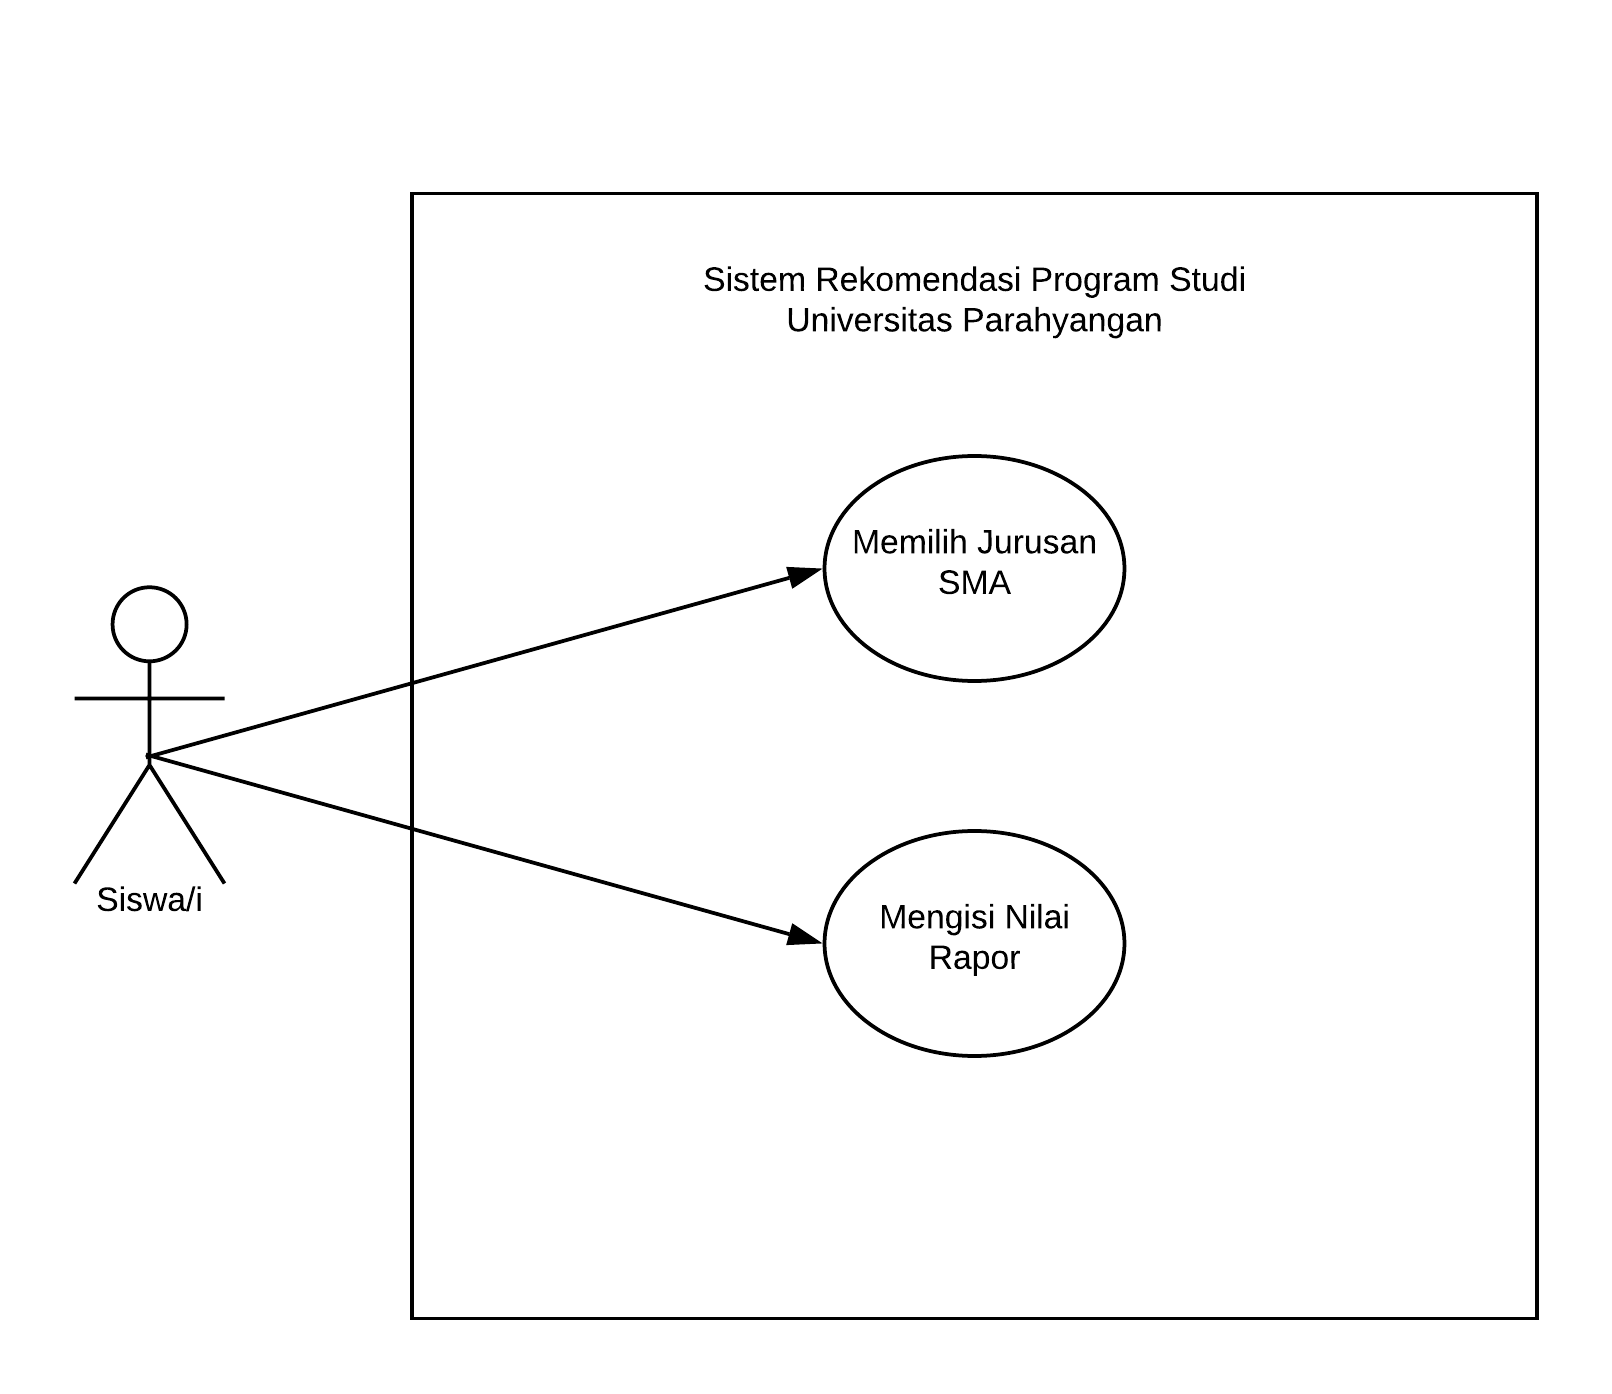
\includegraphics[width = 10cm, height = 10cm]{doc/DokumenSkripsi/Gambar/gambar38.PNG}
                \caption{Hasil Tes \textit{Personal Values}}
                \label{fig:hasil tes personal values}
            \end{figure}
            
    \end{enumerate}
    
    \begin{figure}[H]
        \centering
        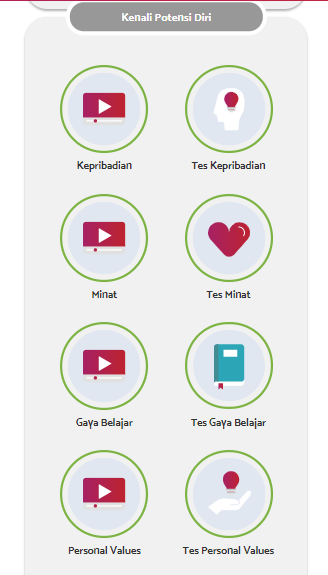
\includegraphics[width = 7cm, height = 11cm ]{Gambar/gambar34.PNG}
        \caption{Modul Potensi Diri}
        \label{fig:modul potensi diri}
    \end{figure}
    
    \item Gambar \ref{fig:modul ukuran kemampuan diri} merupakan modul ketiga setelah modul kenali potensi diri, yaitu modul ukur kemampuan diri. Terdapat beberapa tes yang harus pengguna kerjakan, dengan materi yang berbeda-beda sesuai dengan sub modul yang dikerjakan dan batas waktu yang berbeda-beda. Pengguna dapat melewati pertanyaan yang diberikan. Terdapat 7 sub-modul, yaitu :
    
    \begin{enumerate}
        \item Kemampuan Kognitif \\
             Sub-modul ini merupakan video dengan materi mengukur kemampuan dengan durasi 1 menit 7 detik.
             
        \item Tes Penalaran Induktif \\
            Sub-modul ini terdiri dari dua bagian dengan batas waktu 10 menit dengan materi pengenalan pola untuk mengambil keputusan. Bagian pertama diberikan sebuah pertanyaan dan terdapat empat pilihan jawaban dengan jumlah pertanyaan 11, bagian kedua pertanyaan berupa pola gambar apa di bagian yang kosong dengan jumlah pertanyaan sebanyak 9. 
        
        \item Tes Penalaran Deduktif \\
            Sub-modul ini terdiri dari dua bagian dengan batas waktu 13 menit dengan materi penggnaan fakta yang diketahui untuk mengambil keputusan. Bagian pertama diberikan teka-teki dalam bentuk cerita, pengguna diminta untuk membaca cerita dan menjawab pertanyaan sesuai dengan petunjuk yang diberikan disetiap cerita, dengan jumlah pertanyaan 6. Bagian kedua diberikan teka-teki dalam bentuk gambar, pengguna diminta untuk memilih gambar mana yang sesuai ditempatkan pada bagian yang ditanyakan, dengan jumlah pertanyaan 10.
        
        
        \item Penalaran Angka \\
            Sub-modul ini terdiri sari satu bagian dengan batas waktu 15 menit dengan materi penalaran angka. Pertanyaan berupa deretan angka yang disusun menurut aturan tertentu, pengguna dimina untuk melanjutkan deretan angka tersebut, dengan jumlah pertanyaan 15.
            
        \item Visualisasi \\
            Sub-modul ini terdiri dari satu bagian dengan batas waktu 6 menit 30 detik dengan materi daya bayang bentuk tiga dimensi. Pengguna diminta untuk membayangkan bentuk-bentuk acak tiga dimensi dan menentukan apakah kedua bentuk yang ada pada setiap soal adalah bentuk yang sama atau berbeda dengan jumlah pertanyaan 20.
            
        \item Kecepatan \& Ketelitian \\
            Sub-modul ini terdiri dari dua bagian dengan batas waktu 5 menit dengan materi ketelitian. Pengguna diminta untuk mengurutkan sesuai dengan instruksi yang diberikan dengan jumlah pertanyaan pada bagian pertama 20 dan bagian kedua 25.
        
        \item Pemahaman Bacaan \\
            Sub-modul ini terdiri dari satu bagian dengan batas waktu 15 menit dengan materi pemahaman bacaan. Pengguna diminta untuk membaca sebuah cerita dan menjawab pertanyaan yang berkaitan dengan cerita dengan jumlah pertanyaan 20.
    \end{enumerate}
    
    \begin{figure}[H]
        \centering
        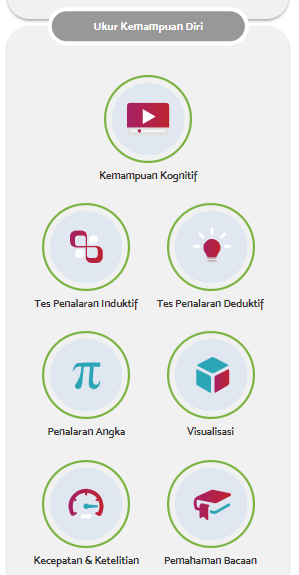
\includegraphics[width = 7cm, height = 11cm ]{Gambar/gambar39.PNG}
        \caption{Modul Ukur Kemampuan Diri}
        \label{fig:modul ukuran kemampuan diri}
    \end{figure}
    
    \item Gambar \ref{fig:hasil rekomendasi} adalah contoh hasil rekomendasikan yang diberikan sistem berdasarkan modul yang sudah dikerjakan. Rekomendasi program studi diberikan setelah pengguna menyelesaikan semua modul yang ada.
    
    \begin{figure}[H]
        \centering
        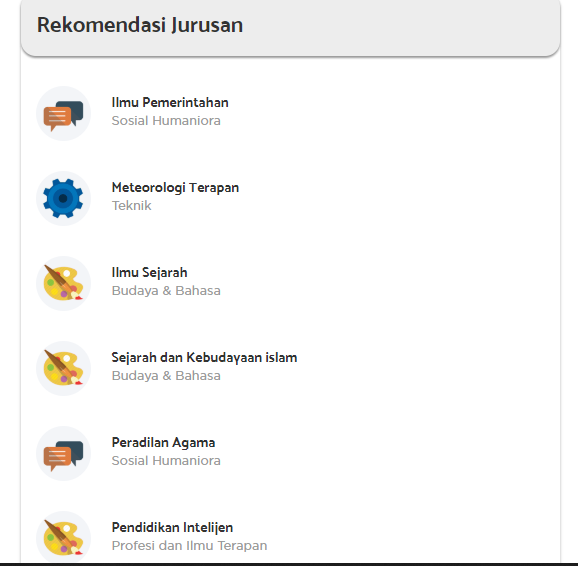
\includegraphics[width = 7cm, height = 10cm ]{Gambar/gambar310.PNG}
        \caption{Hasil Rekomendasi}
        \label{fig:hasil rekomendasi}
    \end{figure}
    
\end{enumerate}

\textit{Website} \url{https://rencanamu.id} memiliki alur program yang pajang sampai pengguna mendapatkan hasil rekomendasi program studi apa yang sesuai. Pengguna harus melakukan login kedalam sistem, mengisi beberapa data diri, dan mengerjakan modul yang didalamnya terdapat beberapa sub-modul. Pengerjaan modul dan sub-modul tidak bisa dilakukan secara acak, pengguna harus menyelesaikan modul atau sub-modul sebelumnya. Di setiap sub-modul, terutama sub-modul yang berisikan tes, diberikan beberapa pertanyaan atau pernyataan yang harus diisi oleh pengguna dan diberikan batas waktu untuk pengerjaan. Pengguna dapat untuk tidak mengerjakan soal yang diberikan, tapi hal tersebut kemungkinan akan berpengaruh terhadap hasil rekomendasi yang diberikan. 

Dari analsis yang dilakukan terhadap \textit{website} \url{https://rencanamu.id}, \textit{website} tersebut memiliki kesamaan dengan sistem yang dibangun yaitu memberikan rekomendasi program studi untuk anak SMA. Perbedaannya pada \textit{website} \url{https://rencanamu.id} tidak menampilkan prediksi IPK dan harus mengisi beberapa modul untuk mendapatkan rekomendasi program studi, sedangkan pada \textit{website} yang akan dibangun, pengguna hanya akan diminta untuk mengisi nilai seusai dengan nilai raport.

\section{Analisis Kebutuhan Sistem}
\label{analisis kebutuhan sistem}
Pada sistem yang akan dibangun, memiliki kebutuhan-kebutuhan perangkat lunak seperti : \textit{Use Case} dan Rancangan Basis Data.

% perlu atau engga ? kata bu mar ga terlalu perlu
\subsection{Diagram \textit{Use Case}}
Pada sistem yang akan dibangun terdapat satu aktor yaitu Siswa/i. Siswa/i ini adalah calon mahasiswa kelas XI yang merupakan target dari sistem yang akan dibangun. Terdapat 4 langkah yang harus dilakukan, yaitu :

\begin{enumerate}
    \item Pendefinisian Aktor
    
    \begin{table}[H]
        \centering
        \begin{tabular}{|c|p{4cm}|p{8cm}|}
            \hline
            No & Aktor & Deskripsi  \\
            \hline
            1 & Siswa/i &  Siswa/i adalah orang yang akan diberikan rekomendasi program studi yang ada di Universitas Parahyangan.\\
            \hline
        \end{tabular}
        \caption{Pendefinisian Aktor}
        \label{tab:pendefsian aktor}
    \end{table}
    
    \item Pendefinisian \textit{Use Case}
    
    \begin{longtable}[H]{|c|p{4cm}|p{8cm}|}
        %\centering
        %\begin{tabular}
            \hline
            No & \textit{Use Case} & Deskripsi  \\
            1 & Memilih Jurusan SMA & Merupakan proses untuk memilih jurusan saat SMA. \\
            \hline
            2 & Mengisi Nilai Rapor & Merupakan proses untuk mengisi nilai beberapa nilai mata pelajaran sesuai dengan jurusan saat SMA. \\ 
            \hline
        %\end{tabular}
        \caption{Pendefinisian \textit{Use Case}}
        \label{tab:pendefinisian use case}
    \end{longtable}
    
    \item Pembuatan \textit{Use Case} Skenario
    
    \begin{longtable}[H]{|p{6.5cm}|p{6.5cm}|}
        %\centering
        %\begin{tabular}
            \hline
            Aksi Aktor & Reaksi Sistem \\
            \hline
            \multicolumn{2}{|c|}{Skenario Normal}\\
            \hline
            1. Memilih jurusan saat SMA. & \\
            \hline
             & 2. Mengarahkan kepada form sesuai jurusan SMA. \\
            \hline
        %\end{tabular}
        \caption{Skenario Memilih Jurusan SMA}
        \label{tab:skenario memilih jurusan sma}
    \end{longtable}
    
    \begin{longtable}[H]{|p{6.5cm}|p{6.5cm}|}
        %\centering
        %\begin{tabular}
            \hline
            \multicolumn{2}{|c|}{Skenario Normal}\\
            \hline
            1. Mengisi nilai sesuai nilai rapor. & \\
            \hline
            & 2. Memeriksa valid tidaknya data yang dimasukkan. \\
            \hline
            & 3. Memeriksa range nilai.\\
            \hline
            4. Klik tombol submit. & \\
            \hline
            & 5. Mengarahkan kepada halaman hasil rekomendasi.\\
            \hline
            \multicolumn{2}{|c|}{Skenario Alternatif}\\
            \hline
             1. Mengisi nilai yang tidak valid. & \\
            \hline
            & 2. Memeriksa valid tidaknya data yang dimasukkan. \\
            \hline
            & 3. Memberikan pesan data tidak valid.\\
            \hline
            4. Mengisi nilai sesuai nilai rapor yang valid. & \\
            \hline
            & 5. Memeriksa \textit{range} nilai.\\
            \hline
            & 6. Memberikan pesan \textit{range} tidak sesuai.\\
            \hline
            7. Mengisi nilai sesuai \textit{range}. &\\
            \hline
            & 8. Memeriksa \textit{range} nilai.\\
            \hline
            9. Klik tombol submit. & \\
            \hline
            & 10. Mengarahkan kepada \textit{page} hasil rekomendasi.\\
            \hline
        %\end{tabular}
        \caption{Skenario Mengisi Nilai Rapor}
        \label{tab:skenario mengisi nilai rapor}
    \end{longtable}
    
    \item Menggambarkan Diagram \textit{Use Case}
    
    \begin{figure}[H]
        \centering
        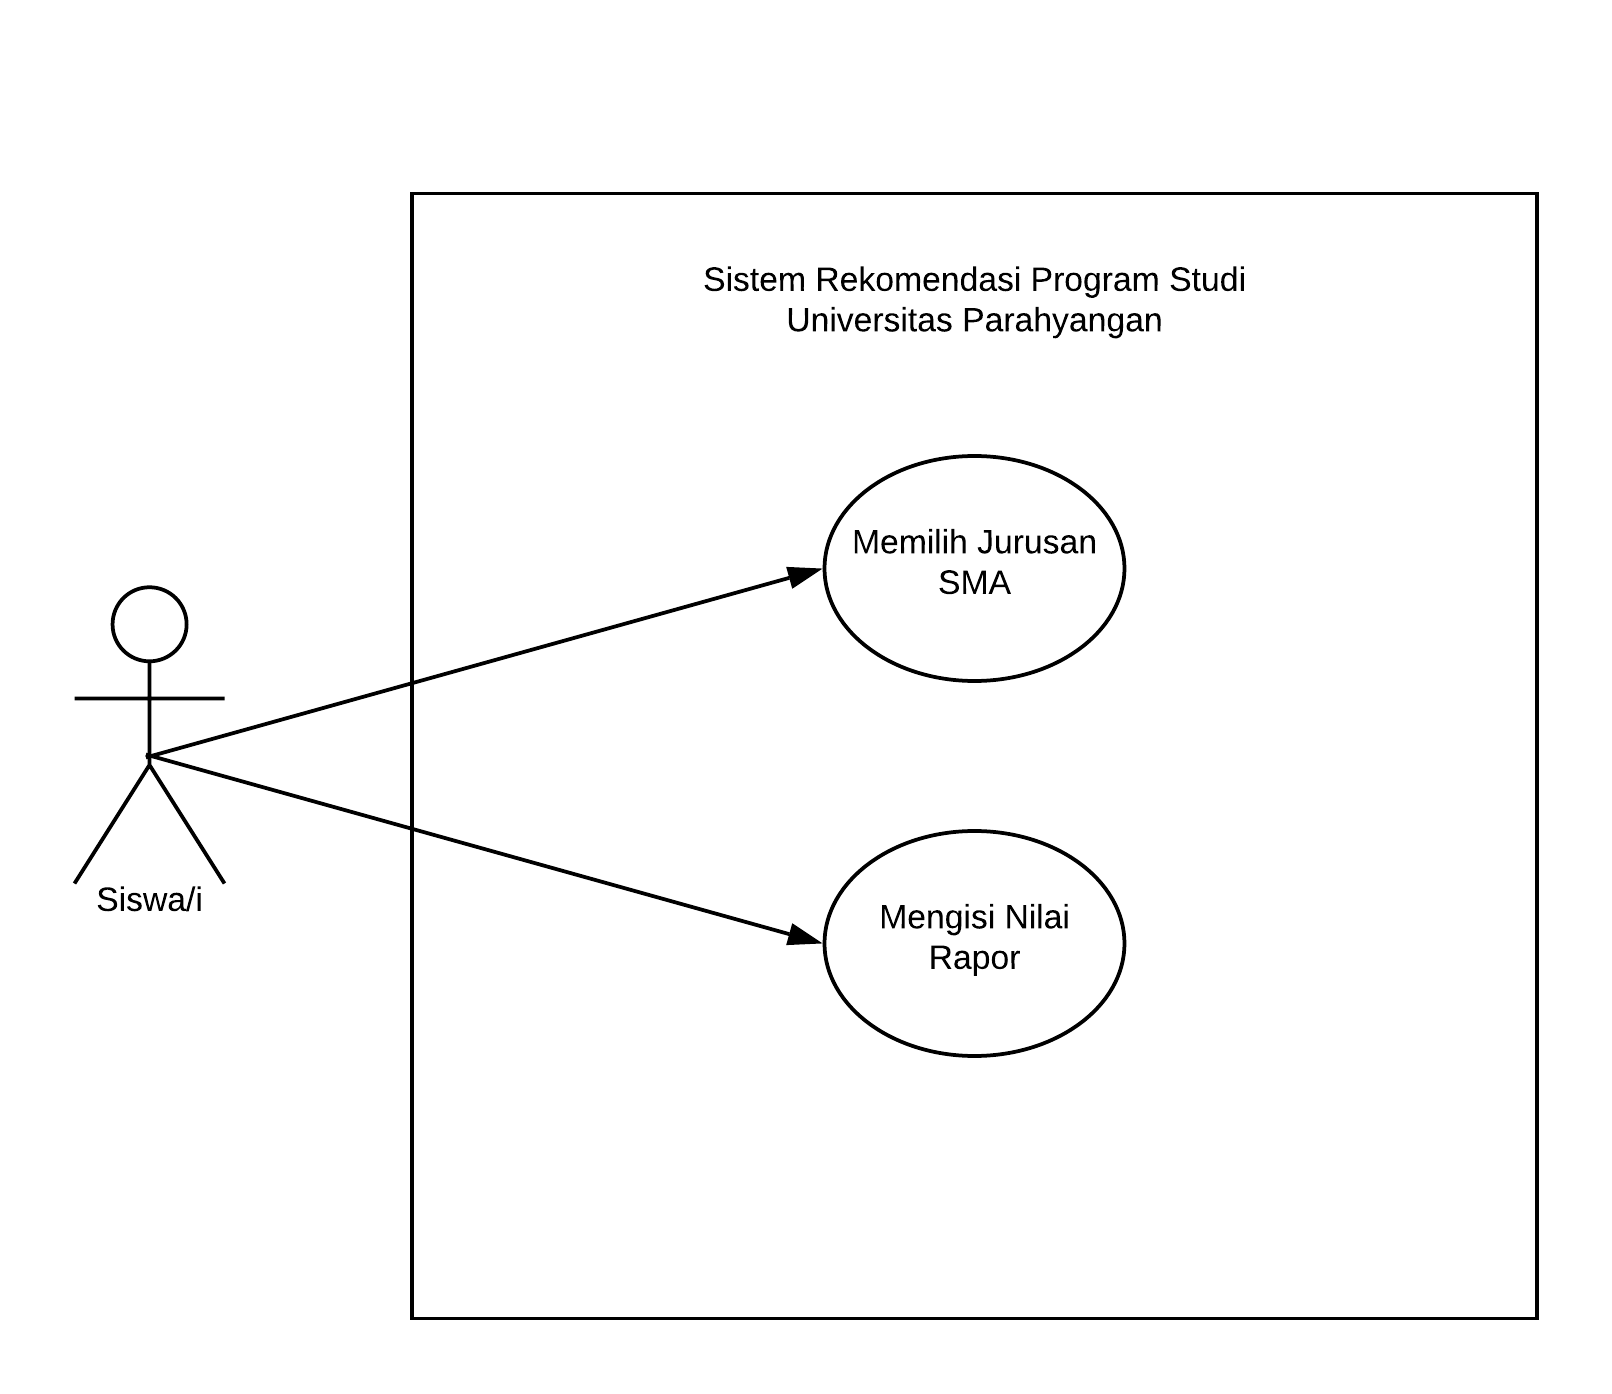
\includegraphics[width = 14cm, height = 14cm]{Gambar/gambar311.png}
        \caption{Diagram \textit{Use Case} Sistem Rekomendasi}
        \label{fig:diagram use case}
    \end{figure}
\end{enumerate}

\subsection{Rancangan Basis Data}
\label{rancangan basis data}
% erd, table, skema relasi

\subsubsection{Diagram ERD}
\label{diagram erd}

\begin{figure}[H]
    \centering
    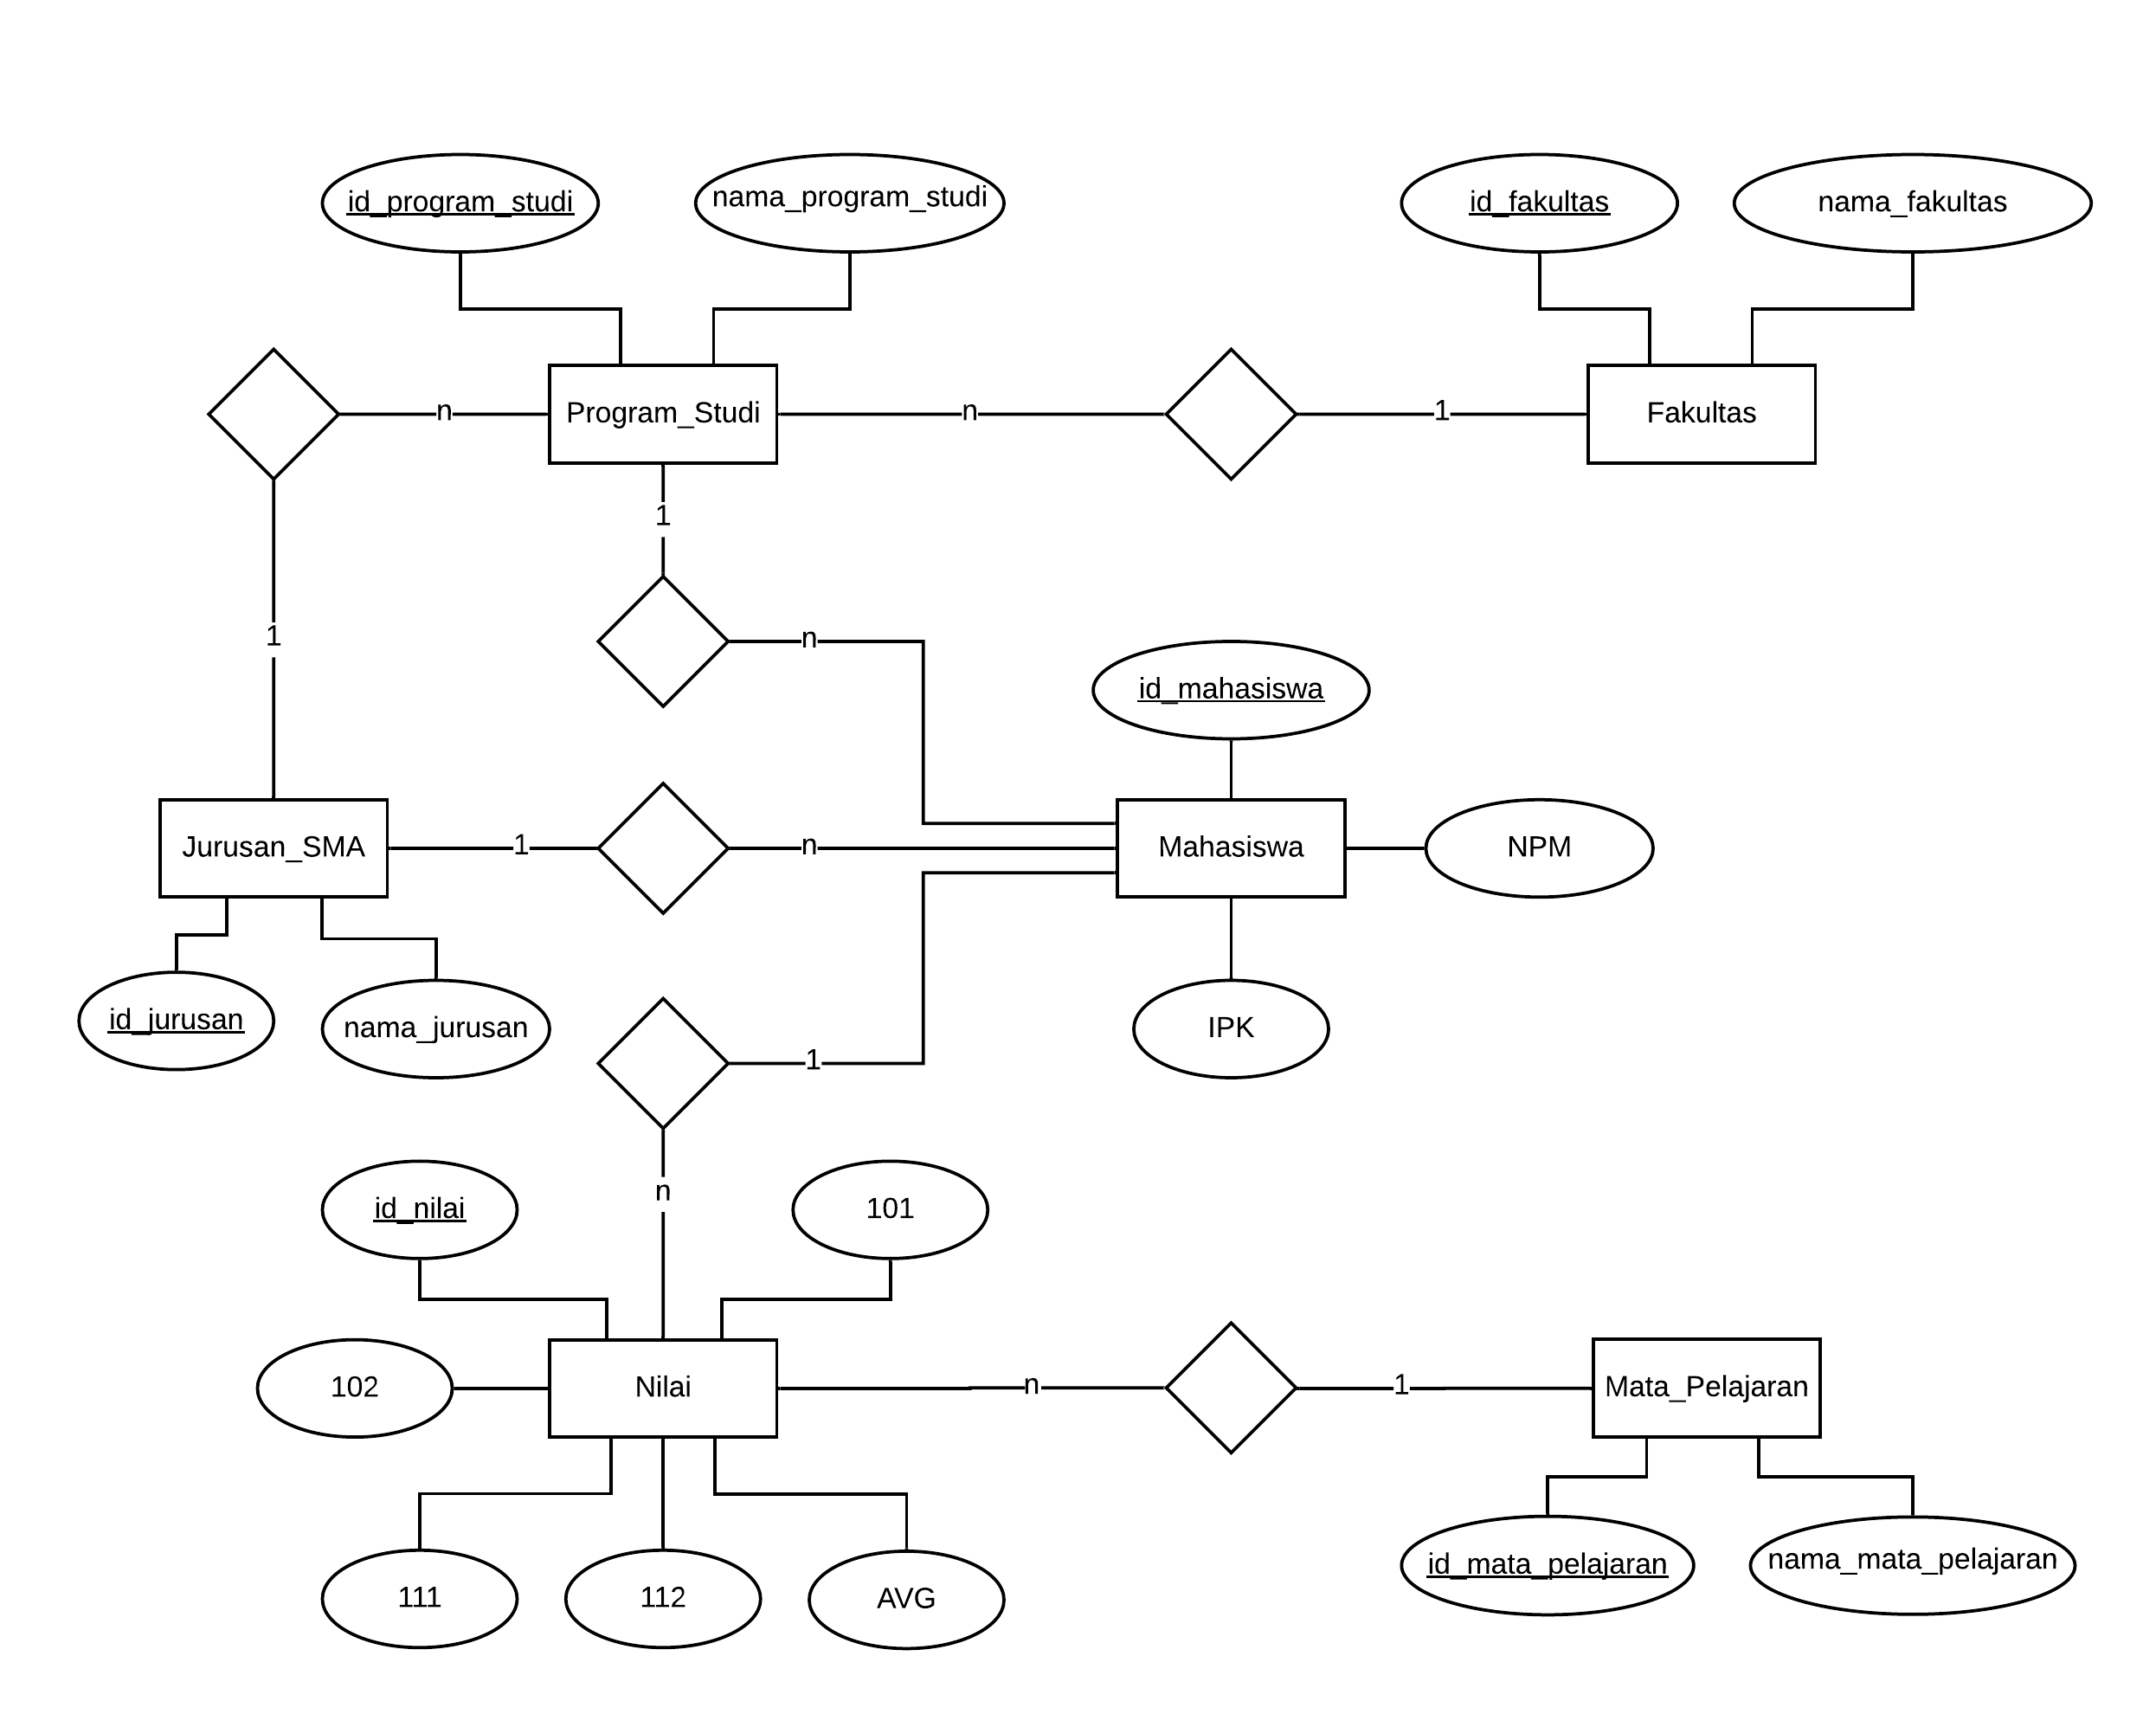
\includegraphics[width = 16cm, height = 14cm ]{Gambar/gambar312.png}
    \caption{Diagram ERD Sistem Rekomendasi}
    \label{fig:diagram erd}
\end{figure}

Berikut merupakan entitas dan atribut gambar \ref{fig:diagram erd} yang akan digunakan pada sistem yang akan dibangun :

\begin{enumerate}
    \item Jurusan\_SMA memiliki atribut id\_jurusan dan nama jurusan.
    
    \item Fakultas memiliki atribut id\_fakultas dan nama\_fakultas.
    
    \item Program\_Studi memiliki atribut id\_program\_studi dan nama\_program\_studi.
    
    \item Mahasiswa memiliki atribut id\_mahasiswa, NPM, dan IPK.
    
    \item Mata\_Pelajaran memiliki atribut id\_mata\_pelajaran dan nama\_mata\_pelajaran.
    
    \item Nilai memiliki atribut id\_nilai, 101, 102, 111, 112, dan AVG. 
\end{enumerate}



